\begin{enumerate}
% rel
\item $M \to M_1$ es $\lambda .P \, 0 \to P$
\begin{figure}[h]
\centering
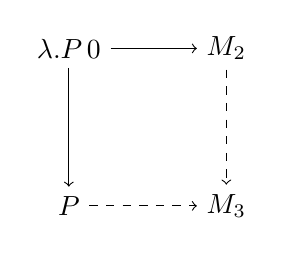
\begin{tikzpicture}
  \node (A) at (0, 2) {$\lambda .P \, 0$};
  \node (B) at (2, 2) {$M_2$};
  \node (C) at (0, 0) {$P$};
  \node (D) at (2, 0) {$M_3$};
  \draw[->]        (A) -- (B);
  \draw[->]        (A) -- (C);
  \draw[->, dashed](B) -- (D);
  \draw[->, dashed](C) -- (D);
\end{tikzpicture}
\end{figure}

\begin{enumerate}
\item $\lambda .P \, 0 \to M_2$ donde $M_2$ es $P$
% es $\lambda .P \, 0 \to P$
\begin{figure}[h]
\centering
\begin{tikzpicture}
  \node (A) at (0, 2) {$\lambda .P \, 0$};
  \node (B) at (2, 2) {$P$};
  \node (C) at (0, 0) {$P$};
  \node (D) at (2, 0) {$M_3$};
  \draw[->]        (A) -- (B);
  \draw[->]        (A) -- (C);
  \draw[->, dashed](B) -- (D);
  \draw[->, dashed](C) -- (D);
\end{tikzpicture}
\end{figure}
Por lo tanto, $M_3$ es $P$.


\item $\lambda .P \, 0 \to M_2$ donde $M_2$ es $\lambda . P_1 \, 0$
% es $\lambda .P \, 0 \to \lambda . P_1 \, 0$
dado que $P \to P_1$ por inversi\'on.
\begin{figure}[h]
\centering
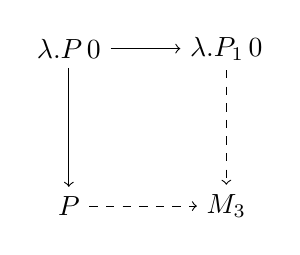
\begin{tikzpicture}
  \node (A) at (0, 2) {$\lambda .P \, 0$};
  \node (B) at (2, 2) {$\lambda . P_1 \, 0$};
  \node (C) at (0, 0) {$P$};
  \node (D) at (2, 0) {$M_3$};
  \draw[->]        (A) -- (B);
  \draw[->]        (A) -- (C);
  \draw[->, dashed](B) -- (D);
  \draw[->, dashed](C) -- (D);
\end{tikzpicture}
\end{figure}
Por $P \to P_1$ entonces $M_3$ es $P_1$ y la reducci\'on de
$\lambda . P_1 \, 0$ es $P_1$.
\end{enumerate}



\newpage
% appL 
\item $M \to M_1$ es $PZ \to P_1 Z$
\begin{figure}[h]
\centering
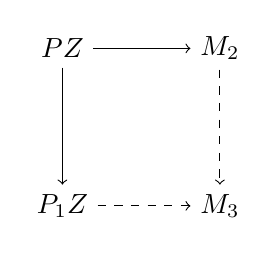
\begin{tikzpicture}
  \node (A) at (0, 2) {$PZ$};
  \node (B) at (2, 2) {$M_2$};
  \node (C) at (0, 0) {$P_1 Z$};
  \node (D) at (2, 0) {$M_3$};
  \draw[->]        (A) -- (B);
  \draw[->]        (A) -- (C);
  \draw[->, dashed](B) -- (D);
  \draw[->, dashed](C) -- (D);
\end{tikzpicture}
\end{figure}

Hipótesis de inducción:
\begin{figure}[h]
\centering
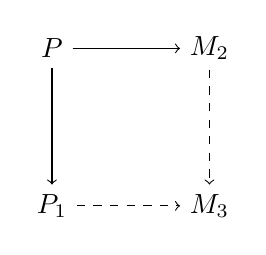
\begin{tikzpicture}
  \node (A) at (0, 2) {$P$};
  \node (B) at (2, 2) {$M_2$};
  \node (C) at (0, 0) {$P_1$};
  \node (D) at (2, 0) {$M_3$};
  \draw[->]        (A) -- (B);
  \draw[->]        (A) -- (C);
  \draw[->, dashed](B) -- (D);
  \draw[->, dashed](C) -- (D);
\end{tikzpicture}
\end{figure}

\begin{enumerate}
\item $PZ \to M_2$ es $PZ \to P_2 Z$
\begin{figure}[h]
\centering
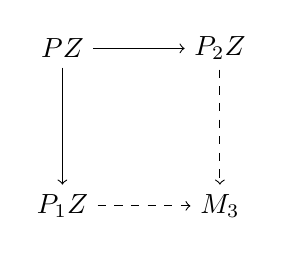
\begin{tikzpicture}
  \node (A) at (0, 2) {$PZ$};
  \node (B) at (2, 2) {$P_2 Z$};
  \node (C) at (0, 0) {$P_1 Z$};
  \node (D) at (2, 0) {$M_3$};
  \draw[->]        (A) -- (B);
  \draw[->]        (A) -- (C);
  \draw[->, dashed](B) -- (D);
  \draw[->, dashed](C) -- (D);
\end{tikzpicture}
\end{figure}
\newpage 

\item $PZ \to M_2$ es $PZ \to P Z_1$
\begin{figure}[h]
\centering
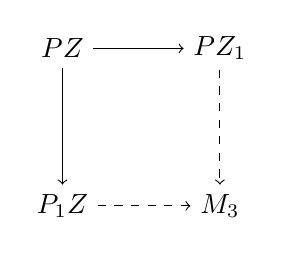
\begin{tikzpicture}
  \node (A) at (0, 2) {$PZ$};
  \node (B) at (2, 2) {$P Z_1$};
  \node (C) at (0, 0) {$P_1 Z$};
  \node (D) at (2, 0) {$M_3$};
  \draw[->]        (A) -- (B);
  \draw[->]        (A) -- (C);
  \draw[->, dashed](B) -- (D);
  \draw[->, dashed](C) -- (D);
\end{tikzpicture}
\end{figure}
\end{enumerate}
% appR
\item $M \to M_1$ es $ZP \to ZP_1$
\begin{figure}[h!]
\centering
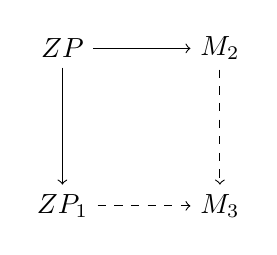
\begin{tikzpicture}
  \node (A) at (0, 2) {$ZP$};
  \node (B) at (2, 2) {$M_2$};
  \node (C) at (0, 0) {$Z P_1$};
  \node (D) at (2, 0) {$M_3$};
  \draw[->]        (A) -- (B);
  \draw[->]        (A) -- (C);
  \draw[->, dashed](B) -- (D);
  \draw[->, dashed](C) -- (D);
\end{tikzpicture}
\end{figure}

Hipótesis de inducción:
\begin{figure}[h]
\centering
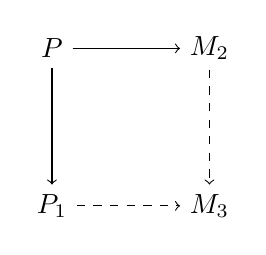
\begin{tikzpicture}
  \node (A) at (0, 2) {$P$};
  \node (B) at (2, 2) {$M_2$};
  \node (C) at (0, 0) {$P_1$};
  \node (D) at (2, 0) {$M_3$};
  \draw[->]        (A) -- (B);
  \draw[->]        (A) -- (C);
  \draw[->, dashed](B) -- (D);
  \draw[->, dashed](C) -- (D);
\end{tikzpicture}
\end{figure}

\newpage 

\begin{enumerate}
\item $ZP \to M_2$ es $ZP \to Z_1 P$
\begin{figure}[h]
\centering
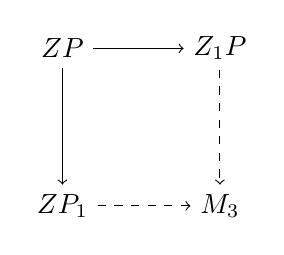
\begin{tikzpicture}
  \node (A) at (0, 2) {$ZP$};
  \node (B) at (2, 2) {$Z_1 P$};
  \node (C) at (0, 0) {$Z P_1$};
  \node (D) at (2, 0) {$M_3$};
  \draw[->]        (A) -- (B);
  \draw[->]        (A) -- (C);
  \draw[->, dashed](B) -- (D);
  \draw[->, dashed](C) -- (D);
\end{tikzpicture}
\end{figure}



\item $ZP \to M_2$ es $ZP \to Z P_2$
\begin{figure}[h]
\centering
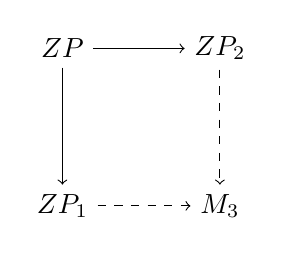
\begin{tikzpicture}
  \node (A) at (0, 2) {$ZP$};
  \node (B) at (2, 2) {$Z P_2$};
  \node (C) at (0, 0) {$Z P_1$};
  \node (D) at (2, 0) {$M_3$};
  \draw[->]        (A) -- (B);
  \draw[->]        (A) -- (C);
  \draw[->, dashed](B) -- (D);
  \draw[->, dashed](C) -- (D);
\end{tikzpicture}
\end{figure}
\end{enumerate}

% xi 
\item $M \to M_1$ es $\lambda .P  \to \lambda . P_1$
\begin{figure}[h]
\centering
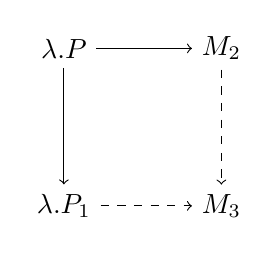
\begin{tikzpicture}
  \node (A) at (0, 2) {$\lambda .P $};
  \node (B) at (2, 2) {$M_2$};
  \node (C) at (0, 0) {$ \lambda . P_1$};
  \node (D) at (2, 0) {$M_3$};
  \draw[->]        (A) -- (B);
  \draw[->]        (A) -- (C);
  \draw[->, dashed](B) -- (D);
  \draw[->, dashed](C) -- (D);
\end{tikzpicture}
\end{figure}

\newpage

Hipótesis de inducción:
\begin{figure}[h]
\centering
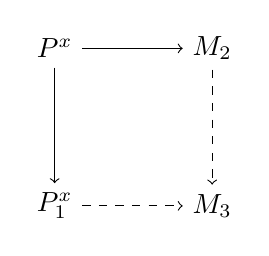
\begin{tikzpicture}
  \node (A) at (0, 2) {$P^x$};
  \node (B) at (2, 2) {$M_2$};
  \node (C) at (0, 0) {$P_1^{x}$};
  \node (D) at (2, 0) {$M_3$};
  \draw[->]        (A) -- (B);
  \draw[->]        (A) -- (C);
  \draw[->, dashed](B) -- (D);
  \draw[->, dashed](C) -- (D);
\end{tikzpicture}
\end{figure}

\begin{enumerate}
\item $\lambda . P  \to M_2$ es $\lambda . M_2 \, 0 \to M_2$
\begin{figure}[h]
\centering
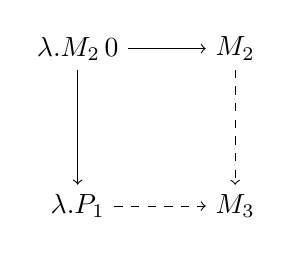
\begin{tikzpicture}
  \node (A) at (0, 2) {$\lambda . M_2 \, 0$};
  \node (B) at (2, 2) {$M_2$};
  \node (C) at (0, 0) {$\lambda . P_1$};
  \node (D) at (2, 0) {$M_3$};
  \draw[->]        (A) -- (B);
  \draw[->]        (A) -- (C);
  \draw[->, dashed](B) -- (D);
  \draw[->, dashed](C) -- (D);
\end{tikzpicture}
\end{figure}

\item $\lambda .P \to M_2$ es $\lambda .P \to \lambda . P_2 $
\begin{figure}[h]
\centering
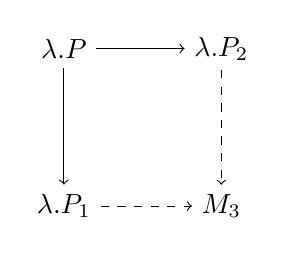
\begin{tikzpicture}
  \node (A) at (0, 2) {$\lambda .P $};
  \node (B) at (2, 2) {$\lambda . P_2$};
  \node (C) at (0, 0) {$\lambda . P_1$};
  \node (D) at (2, 0) {$M_3$};
  \draw[->]        (A) -- (B);
  \draw[->]        (A) -- (C);
  \draw[->, dashed](B) -- (D);
  \draw[->, dashed](C) -- (D);
\end{tikzpicture}
\end{figure}
\end{enumerate}

\end{enumerate}
